
\chapter{Week 6}

\section{Monday}\index{Monday_lecture}

\subsection{Conditional Expectation}

Consider the probability space $(\Omega,\mathcal{F},\mathbb{P})$,
where the $\sigma$-field $\mathcal{F}$ represents the collection of all information
to be measured.

In practice, we often meet the situation that the information is partially available.
This can be represented by $\mathcal{G}$, another $\sigma$-field but a subset of $\mathcal{F}$.
We call $\mathcal{G}$ a sub-$\sigma$-field.

\begin{definition}[Partition]
We call $\mathcal{A}\triangleq\{A_i\in\mathcal{F}; i\ge1\}$ a partition of $\Omega$ if
\[
A_i\cap A_j=\emptyset, \forall i\ne j,\quad
\text{ and }\quad \bigcup_{i=1}^\infty A_i=\Omega.
\]
\end{definition}
Denote the minimal $\sigma$-field on $\Omega$ containing $\mathcal{A}$ by $\sigma(\mathcal{A})$,
which is a sub-$\sigma$-field, and it is easy to show that 
\[
\sigma(\mathcal{A}) = \left\{
\bigcup_{i\in B}A_i:~B\subseteq\mathbb{N}
\right\}.
\]
The partition $\{A_i\in\mathcal{F}; i\ge1\}$ denotes the set of minimal information units for $\sigma(\mathcal{A})$.

The expectation $\mathbb{E}[X]$ can be considered as the prediction of $X(\omega)$ under no information on the sample $\omega\in\Omega$.
Instead, if we have some information about $\omega$, e.g., $\omega\in A_1$ for $A_1\in\mathcal{F}$ and $\mathbb{P}(A_1)>0$,
then the prediction of $X$ given $A_1$ is defined as
\[
\mathbb{E}[X\mid A_1]\triangleq \frac{\mathbb{E}[X1_{A_1}]}{\mathbb{P}(A_1)}.
\]
We call it the \emph{conditional expectation of $X$ given $A_1$}.

Based on this definition, we can define conditional expectation given a simple $\sigma$-field.
For $A_1\in\mathcal{F}, A_2=A_1^c$, set $\mathcal{G}=\{\emptyset,A_1,A_2,\Omega\}$.
Then define the \emph{conditional expectation of $X$ given $\mathcal{G}$} as
\begin{equation}\label{Eq:6:1}
\mathbb{E}[X\mid \mathcal{G}](\omega)=\left\{
\begin{aligned}
\mathbb{E}[X\mid A_1]1(\mathbb{P}(A_1)>0),&\quad\text{for $\omega\in A_1$}\\
\mathbb{E}[X\mid A_2]1(\mathbb{P}(A_2)>0),&\quad\text{for $\omega\in A_2$}
\end{aligned}
\right.
\end{equation}
The following presents an image of conditional expectation given $\sigma(\mathcal{A})$, where $\mathcal{A}$ is a partition:
\begin{figure}[H]
\centering
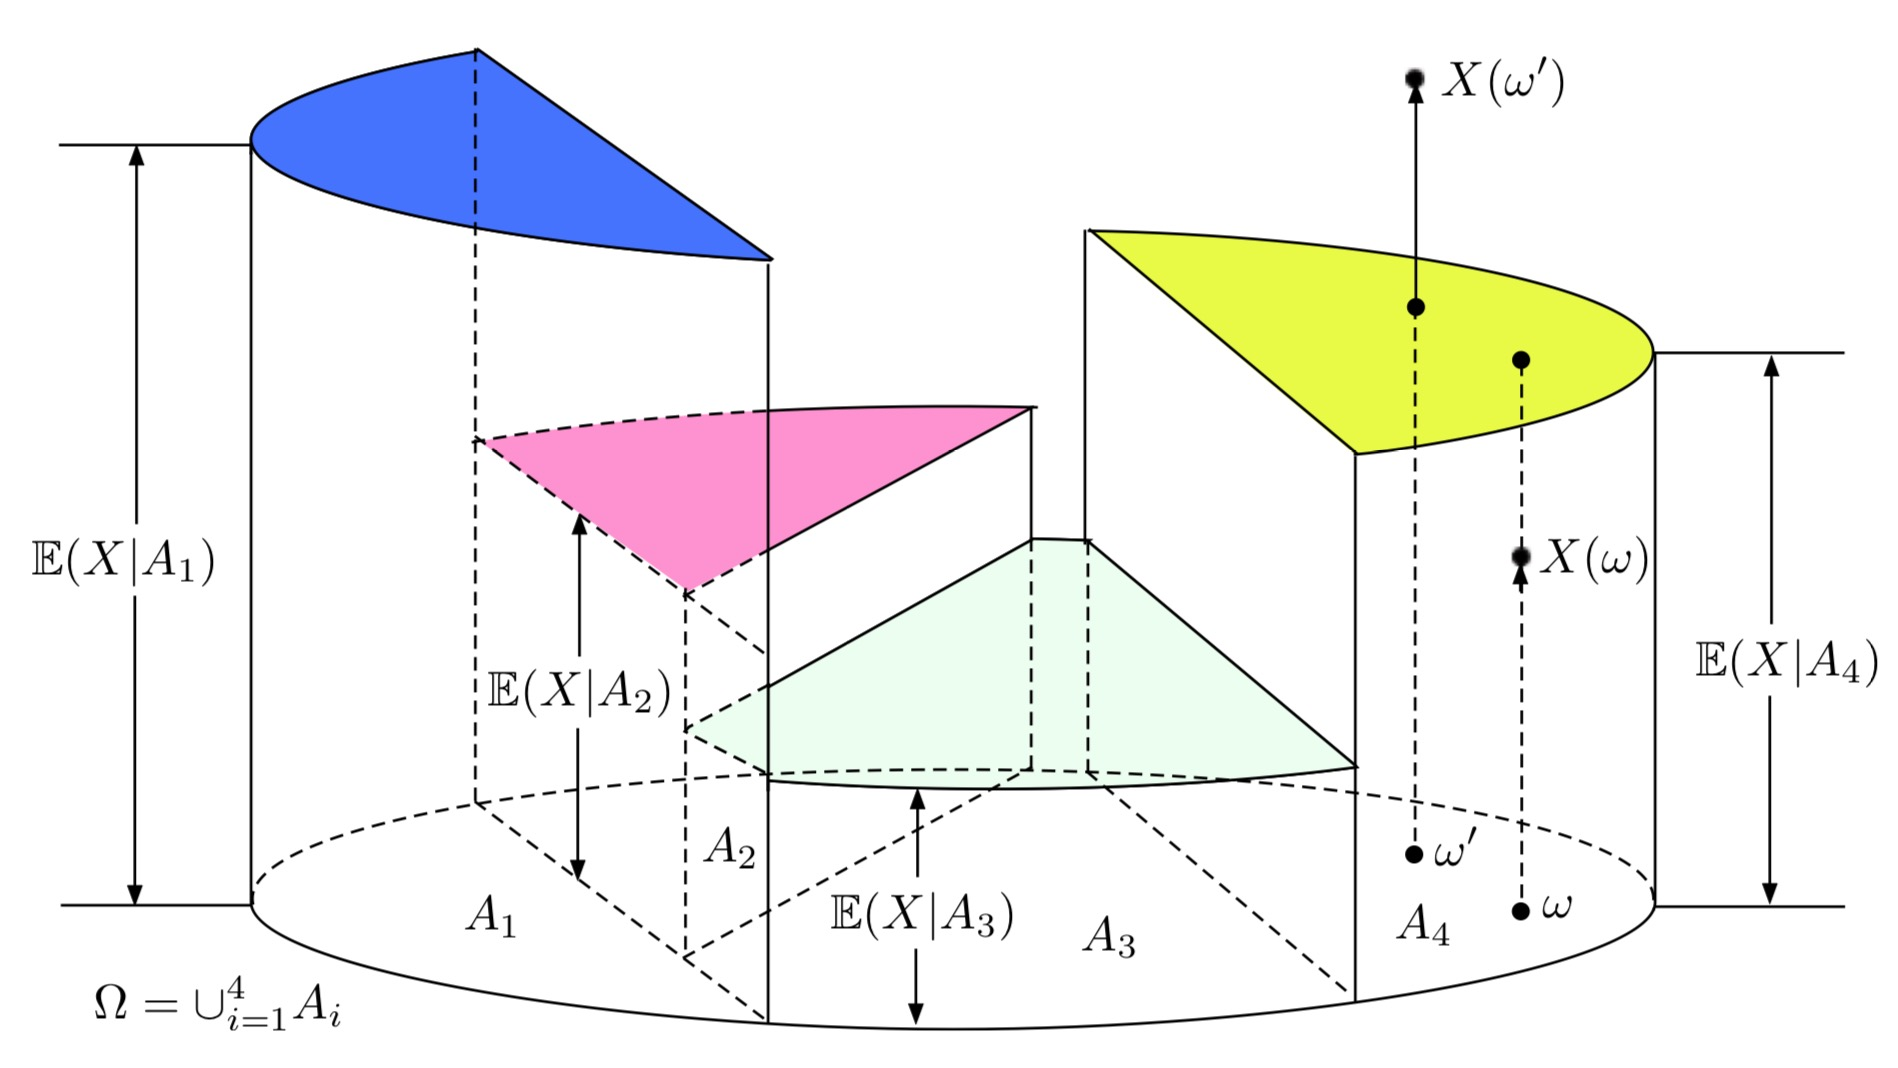
\includegraphics[width=0.8\textwidth]{week6/p_2}
\caption{Illustration of $\mathbb{E}[X\mid \sigma(\mathcal{A})]$,
where $\mathcal{A}=\{A_i\in\mathcal{F};~\cup_iA_i=\Omega\}$.
}
\end{figure}
We extend the definition in (\ref{Eq:6:1}) to general $\sigma$-field:
\begin{definition}\label{Def:6:2}
Given an integrable random variable and a sub $\sigma$-field $\mathcal{G}$, 
we say $Z$ is the conditional expectation of $X$ given $\mathcal{G}$, denoted by $\mathbb{E}[X\mid \mathcal{G}]$, if
\begin{enumerate}
\item
$Z$ is $\mathcal{G}$-measurable;
\item
For any $A\in\mathcal{G}$, $\mathbb{E}[Z1_A] = \mathbb{E}[X1_A]$.
\end{enumerate}
\end{definition}
The existence of such $Z$ is because of Radon-Nikodym theorem. Intuitively, this can be seen by approximating $\mathcal{G}$ from partitions.

\begin{theorem}[Uniqueness of Conditional Expectation]
Under the setting of Definition~\ref{Def:6:2},
suppose that $Z_1,Z_2$ satisfies the condition 1) and 2), then 
$Z_1=Z_2$ a.s.
\end{theorem}
\begin{proof}
Let $A=\{Z_1-Z_2>0\}\in\mathcal{G}$, then by condition 2) in Definition~\ref{Def:6:2},
\[
\mathbb{E}[(Z_1-Z_2)1_A] = \mathbb{E}[Z_11_A] - \mathbb{E}[Z_21_A] = 
\mathbb{E}[X1_A]-\mathbb{E}[X1_A]=0.
\]
This equality implies that $\mathbb{P}(A)=0$. Similarly, $\mathbb{P}(Z_2-Z_1>0)=0$.
The proof is complete.
\end{proof}

\begin{remark}
Since $\mathbb{E}[X\mid \mathcal{G}]$ is uniquely determined a.s., in what follows, we omit a.s. unless otherwise stated.
\end{remark}

\begin{proposition}[Basic properties of the conditional expectation]\quad
\begin{enumerate}
\item
\[
\mathbb{E}(\mathbb{E}[X\mid \mathcal{G}]) = \mathbb{E}[X]
\]
\item
\[
\mathbb{E}[aX+bY\mid \mathcal{G}] = a\mathbb{E}[X\mid \mathcal{G}] + b\mathbb{E}[Y\mid \mathcal{G}]
\]
\item
If $X$ and $\mathcal{G}$ are independent, i.e., for any $B\in\mathcal{B}(\mathbb{R})$ and $A\in\mathcal{G}$,
the events $\{X\in B\}$ and $A$ are independent, then
\[
\mathbb{E}[X\mid \mathcal{G}] = \mathbb{E}[X]
\]
\item
If $Y$ is $\mathcal{G}$-measurable and $\mathbb{E}|X|,\mathbb{E}|XY|<\infty$, then
\[
\mathbb{E}[XY\mid \mathcal{G}] = \mathbb{E}[X\mid \mathcal{G}]Y.
\]
\end{enumerate}
\end{proposition}

Now we can also define the conditional expectation given a random variable as the following:
\begin{definition}[Conditional Expectation given a Random Variable]
Given a random variable $Y$, define the generated $\sigma$-field
\[
\sigma(Y)\triangleq\{\{Y\in B\}:~B\in\mathcal{B}(\mathbb{R})\}.
\]
The conditional expectation of $X$ given $Y$, denoted as $\mathbb{E}[X\mid Y]$, is defined as
\[
\mathbb{E}[X\mid Y]\triangleq\mathbb{E}[X\mid \sigma(Y)].
\]
\end{definition}

\begin{definition}[Conditional Probability]
Given $A\in\mathcal{F}$ and a sub-$\sigma$-field $\mathcal{G}$, define the 
\emph{conditional probability of $A$ given $\mathcal{G}$} as
\[
\mathbb{P}(A\mid \mathcal{G})\triangleq\mathbb{E}[1_A\mid \mathcal{G}].
\]
In particular, for a random variable $Y$,
\[
\mathbb{P}(A\mid Y)\triangleq\mathbb{E}[1_A\mid\sigma(Y)]
\]
is called the \emph{conditional probability of $A$ given $Y$}.
\end{definition}

The conditional expectation $\mathbb{E}[X\mid \mathcal{G}]$ minimizes the expected squared error to estimate $X$ among all $\mathcal{G}$-measurable random variables, when $\mathbb{E}[X^2]<\infty$.
\begin{theorem}[Minimizing Squared Error]
For a random variable and sub $\sigma$-field $\mathcal{G}$, assume that $\mathbb{E}[X^2]<\infty$.
Then, for  $\mathcal{G}$-measurable random variable $Z$,
$\mathbb{E}[(X-Z)^2]$ is minimized by $Z=\mathbb{E}[X\mid\mathcal{G}]$.
\end{theorem}
\begin{proof}
Expand $\mathbb{E}[(X-Z)^2]$ as the following:
\begin{align*}
\mathbb{E}[(X-Z)^2]&=\mathbb{E}[(X-\mathbb{E}[X\mid\mathcal{G}]+\mathbb{E}[X\mid\mathcal{G}]-Z)^2]\\
&=\mathbb{E}[(X-\mathbb{E}[X\mid\mathcal{G}])^2] + \mathbb{E}[(\mathbb{E}[X\mid\mathcal{G}]-Z)^2]+ 2\mathbb{E}[
(X-\mathbb{E}[X\mid\mathcal{G}])(\mathbb{E}[X\mid\mathcal{G}]-Z)
]
\end{align*}
In particular, for $\mathcal{G}$-measurable random variable $H$,
\[
H\mathbb{E}[X\mid\mathcal{G}] = \mathbb{E}[HX\mid\mathcal{G}]\implies
\mathbb{E}[H\mathbb{E}[X\mid\mathcal{G}]]=\mathbb{E}[HX]
\]
As a result, $\mathbb{E}[(X-\mathbb{E}[X\mid\mathcal{G}])H]=0$. Hence
\[
\mathbb{E}[(X-Z)^2] = \mathbb{E}[(X-\mathbb{E}[X\mid\mathcal{G}])^2] + \mathbb{E}[(\mathbb{E}[X\mid\mathcal{G}]-Z)^2].
\]
This objective is minimized by $Z=\mathbb{E}[X\mid\mathcal{G}]$.
\end{proof}

\subsection{Discrete Time Stochastic Process}
\begin{definition}[Stochastic Process]
\begin{itemize}
\item
Consider the topological space $(S,\mathcal{O})$, define 
\[
\mathcal{B}(S^n) = \sigma(\mathcal{O}^n).
\]
\item
The discrete time stochastic process with state space $S$ is defined as 
\[
X_{\cdot}=\{X_n:\Omega\to S:~n\ge0 \}.
\]
For each $\omega\in\Omega$, $X_{\cdot}(\omega)\triangleq\{X_n(\omega):~n\ge0\}$ is called a sample path.
\item
For $n\ge0$, let $\mathcal{F}_n^X\triangleq \{
\{(X_0,X_1,\ldots,X_n)\in\bm B\}:~\bm B\in \mathcal{B}(S^n)
\}$, which is a sub $\sigma$-field of $\mathcal{F}$, which presents all information generated by $X_0,X_1,\ldots,X_n$.
\end{itemize}
\end{definition}

A collection of sample paths is called a history of $X_{\cdot}$.
The sub $\sigma$-field $\mathcal{F}_n^X$ can be viewed as the observation on the history of $X_{\cdot}$ up to $n$.

\begin{definition}[Filtration]
A sequence of sub $\sigma$-fields, $\mathbb{F}\triangleq \{\mathcal{F}_n:~n\ge\}$,
is called a \emph{filtration} if $\mathcal{F}_n\subseteq\mathcal{F}_{n+1},\forall n\ge0$.
We say the stochastic process is \emph{adapted} to filtration $\mathbb{F}$ if $\mathcal{F}_n^X\subseteq\mathcal{F}_n,\forall n\ge0$.
The special \emph{filtration}, $\mathbb{F}^X\triangleq \{\mathcal{F}_n^X:~n\ge0\}$, is called the \emph{natural filtration} of $X_{\cdot}$.
\end{definition}

Given a stochastic process $X_{\cdot}$, one may prdict the value of $f(X_{n+1})$ given the information up to time $n$ by
\[
\mathbb{E}[f(X_{n+1})\mid\mathcal{F}_n].
\]
We can also show that
\[\mathbb{E}
[
\mathbb{E}[f(X_{n+2})\mid\mathcal{F}_{n+1}]\mid\mathcal{F}_n
]=\mathbb{E}[f(X_{n+2})\mid\mathcal{F}_{n}],
\]
which means that smaller information makes the conditional expectation smoother as a function of sample $\omega\in\Omega$.

\begin{example}[Random Walk]
Suppose that $U_1,U_2,\ldots$ are i.i.d. with $\mathbb{P}(U_n=1)=p, \mathbb{P}(U_n=-1)=1-p$.
Then define the stochastic process $X_{\cdot}$ with $X_0=0$,
\[
X_n = U_1+U_2+\cdots+U_n,\quad n\ge1.
\]
Then $X_{\cdot}$ is called a simple random walk.
We can see that $X_{\cdot}$ is $\mathbb{F}^X$-adapted, and
\[
\mathbb{E}[X_{n+1}\mid\mathcal{F}_n^X] = X_n + \mathbb{E}[U_{n+1}\mid\mathcal{F}_n^X]=X_n+(p-(1-p)),\quad n\ge0.
\]
\end{example}


\section{Thursday}
\subsection{Markov Process}
Now we study one of the most popular stochastic processes, the Markov processes.
Denote $D_b(S)$ as the set of all bounded measurable functions from $S$ to $\mathbb{R}$.

\begin{definition}[Markov Process]\label{Def:6:7}
A stochastic process $X_{\cdot}$ with state space $S$ is called a \emph{discrete-time Markov process}~(DTMC) for filtration $\mathbb{F}$ if
\begin{enumerate}
\item
$X_{\cdot}$ is adapted to $\mathbb{F}$;
\item
$\mathbb{E}[f(X_{n+1})\mid\mathcal{F}_n] = \mathbb{E}[f(X_{n+1})\mid X_n]$ for any $f\in D_b(S)$ and $n\ge0$.
\end{enumerate}
In particular, if $S$ is countable, then it is called a Markov Chain.
\end{definition}
It is clear that for a Markov Chain $X_{\cdot}$, the second condition is equivalent to 
\[
\mathbb{P}[X_{n+1}=j\mid\mathcal{F}_n] = \mathbb{P}[X_{n+1}=j\mid X_n],\quad j\in S, n\ge0.
\]

\begin{definition}[Time-Homogeneous]
A DTMC $X_{\cdot}$ is said to have \emph{time-homogeneous} transitions if the second condition in Definition~\ref{Def:6:7} is independent of $n$. 
\end{definition}

\begin{definition}[Transition of Markov Chain]
Given a Markov Chain $X_{\cdot}$ with state space $S$, define the transition probability
\[
p_{i,j}(n) = \mathbb{P}[X_{n+1}=j\mid X_n=i],\quad i,j\in S, n\ge0.
\]
Define the transition operator $P_n: D_b(S)\to D_b(S)$ as
\[
P_n[f(i)] = \sum_{j\in S}f(j)p_{i,j}(n),\quad i\in S, f\in D_b(S).
\]
In particular, if the Markov Chain $X_{\cdot}$ has time-homogeneous transitions, the matrix $P=(p_{i,j})_{i,j}$ is called a \emph{transition matrix}.
A directed graph $(V,E)$ with 
\[
V=S,\quad E=\{e_{i,j}:~p_{i,j}>0, i,j\in S\}
\]
is called a \emph{transition diagram}.
\end{definition}

Given a time-homogeneous Markov Chain, define the higher order transitons as the following:
\begin{align*}
p_{i,j}^{(n)}&=\mathbb{P}(X_{n}=j\mid X_0=i),\quad i,j\in S\\
P^{(n)}[f(i)]&=\mathbb{E}[f(X_n)\mid X_0=i],\quad i\in S, f\in D_b(S).
\end{align*}
Because of the time-homogeous transition assumption, for $n,\ell\ge0$,
\begin{align*}
p_{i,j}^{(n)}&=\mathbb{P}(X_{n+\ell}=j\mid X_{\ell}=i),\quad i,j\in S\\
P^{(n)}[f(i)]&=\mathbb{E}[f(X_{n+\ell})\mid X_{\ell}=i],\quad i\in S, f\in D_b(S).
\end{align*}
Define $P^n[f(i)] = \sum_{i\in S}[P^n]_{i,j}f(j)$, then we can show that 
\[
P^{(n)}[f(i)] = P^n[f(i)],\quad i\in S, f\in D_b(S).
\]

\begin{example}
The simple random walk is a Markov chain with state space $\mathbb{Z}$ and natural filtration $\mathbb{F}^X$ since
\[
\mathbb{E}[f(X_{n+1})\mid\mathcal{F}_n^X] = \mathbb{E}[f(X_{n}+U_{n+1})\mid X_n]
\]
The transition probability $p_{i,j}$ is 
\[
p_{i,j} = \mathbb{P}(X_{n+1}=j\mid X_n=i) = p\cdot 1(j=i+1) + (1-p)\cdot 1(j=i-1).
\]
\end{example}

\begin{example}[Stochastic Process generated by i.i.d. Random Variables]
Consider an i.i.d. sequence of random variables $U_n$, define $X_{\cdot}$ with
\[
X_n = g(X_{n-1},U_n).
\]
We can see that $X_{\cdot}$ is a Markov Chain with time-homogeneous transitions for filtration $\mathbb{F}^X$
when $U_n$ is independent of $\mathcal{F}_n^X$
\end{example}

\begin{example}
Suppose that $X_n$ takes values in $\mathbb{Z}_+$ with $X_0=1$, 
\[
X_{n+1} = \sum_{k=1}^{X_n}U_{n,k},\quad n\ge0,
\]
where $U_{n,k}$'s are i.i.d. random variables. 
Then $X_{\cdot}$ is called a \emph{branching process}.
We can see that such a process is a Markov process:
\[
\mathbb{E}[f(X_{n+1})\mid\mathcal{F}_n^X] = \mathbb{E}[f(\sum_{k=1}^{X_n}U_{n,k})\mid X_n]
\]
The transition probability is given by
\[
p_{i,j} = \mathbb{P}\left(
\sum_{k=1}^{i}U_{n,k}\middle| X_n=i
\right).
\]
Take $\lambda = \mathbb{E}[U_{n,k}]$, then
\[
\mathbb{E}[X_{n+1}]=\mathbb{E}[\sum_{k=1}^{X_n}\mathbb{E}[U_{n,k}\mid X_n]] = \lambda\mathbb{E}[X_{n}].
\]
Therefore, $\mathbb{E}[X_{n}]=\lambda^n$.
\end{example}

\subsection{Martingale and Semi-martingale}

\begin{definition}[Predictable]
The stochastic process $X_{\cdot}\triangleq\{X_n:~n\ge0\}$ is said to be $\mathbb{F}$-predictable
for filtration $\mathbb{F}\triangleq\{\mathcal{F}_n:~n\ge0\}$ if 
\begin{enumerate}
\item
$X_0$ is $\mathcal{F}_0$-measurable;
\item
$X_n$ is $\mathcal{F}_{n-1}$-measurable, $\forall n\ge1$.
\end{enumerate}
\end{definition}
Define $E_0=0$ and 
\[
E_n = X_n - \mathbb{E}[X_n\mid \mathcal{F}_{n-1}],\quad n\ge1,
\]
which is an estimation error of $X_n$ given $\mathbb{F}_{n-1}$, the observation by time $n-1$.
Then $X_n$ can be written as
\[
X_n = \mathbb{E}[X_n\mid \mathcal{F}_{n-1}] + E_n,\quad n\ge1.
\]
Then a stochastic process can be decomposed as a predictable process and a martingale:
\[
Y_n = X_0 + \sum_{\ell=1}^n\mathbb{E}[X_\ell-X_{\ell-1}\mid \mathcal{F}_{\ell-1}],\qquad
M_n=\sum_{\ell=1}^nE_{\ell}.
\]
It is easy to see that 
\begin{equation}\label{Eq:6:2}
X_n = Y_n + M_n, n\ge0.
\end{equation}
We can verify that $\{Y_n:~n\ge0\}$ is predictable, while
\[
\mathbb{E}[M_n\mid\mathcal{F}_{n-1}] = \mathbb{E}[M_{n-1}+E_n\mid\mathcal{F}_{n-1}]=M_{n-1}.
\]

\begin{definition}[Martingale]
A real valued stochastic prcoess $M_{\cdot}\triangleq \{M_n:~n\ge0\}$ is called an $\mathbb{F}$-martingale if
\begin{enumerate}
\item
$M_n$ is integrable for all $n$;
\item
$M_{\cdot}$ is adapted to the filtration $\mathbb{F}$;
\item
$\mathbb{E}[M_{n+1}\mid\mathcal{F}_{n}]=M_n,\forall n\ge0$.
\end{enumerate}
If the equality is replaced by ``$\le$'' or ``$\ge$'', then $M_{\cdot}$ is called an $\mathbb{F}$ super-(or sub-) martingale.
\end{definition}

\begin{theorem}[Semi-martingale Representation due to Doob]
An $\mathbb{F}$-adapted process $X_{\cdot}$ with integrable $X_n,\forall n\ge0$ is unquely decomposed in the form of (\ref{Eq:6:2}) almost surely by
an $\mathbb{F}$-predictable process $\{Y_n:~n\ge0\}$ and an  $\mathbb{F}$-martingale $\{M_n:~n\ge0\}$ with $M_n=0$.
The stochastic process $X_{\cdot}$ having this decomposition is called an $\mathbb{F}$-semimartingale.
\end{theorem}
\begin{proof}
Assume on the contrary that there is another decomposition $X_n=Y_n'+M_n'$, then
\[
Y_{n+1}-Y_{n+1}' = \mathbb{E}[Y_{n+1}-Y_{n+1}'\mid\mathcal{F}_n]
=\mathbb{E}[M_{n+1}'-M_{n+1}\mid\mathcal{F}_n]=M_n'-M_n.
\]
Since $M_0'-M_0=0$, we imply $Y_1-Y_n'=0$, which further implies $M_1=M_1'$.
Inductively, the uniqueness is proved.

\end{proof}

\begin{corollary}
If $X_{\cdot}$ is an $\mathbb{F}$-subimartingale,
then the $\mathbb{F}$-predictable component $Y_n$ is non-decreasing in $n$ a.s. for the semi-martingale representation $X_n = Y_n+M_n$.
\end{corollary}
\begin{proof}
By the definition of submartingale,
\[
\mathbb{E}[X_{n+1}\mid\mathcal{F}_n]\ge X_n = Y_n+M_n.
\]
Substituting $X_{n+1}$ with $Y_{n+1}+M_{n+1}$ gives
\[
\mathbb{E}[X_{n+1}\mid\mathcal{F}_n] = Y_{n+1}+M_n.
\]
Thus $Y_{n+1}-Y_n\ge0$.
\end{proof}
In (\ref{Eq:6:2}), $\{E_n:~n\ge1\}$ may be considered as a sequence of white noises,
and $\mathbb{F}$-martingale $M_{\cdot}$ may be interpreted as an accumulated white noise.
We need $M_n$ to be a martingale because:
\begin{enumerate}
\item
It uniquely determines the decomposition;
\item
It extracts the noise component from ongoing history;
\item
It is analytically tractable, enabling us to study various asymptotic problems.
\end{enumerate}

Any discrete-time stochastic process can be viewed as a semi-martingale, but its martingale component may not be easily computed. Here gives several simple cases:
\begin{example}
\begin{itemize}
\item
For simple random walk,
\[
\mathbb{E}[X_{n+1}\mid\mathcal{F}_n] - X_n = \mathbb{E}[U_{n+1}\mid\mathcal{F}_n]=a
\]
\item
Assume that $\mathbb{E}[U_{n}^2]=b<\infty$, then
\[
\mathbb{E}[X_{n+1}^2\mid\mathcal{F}_n] - X_n^2=2aX_n+b.
\]
\end{itemize}
\end{example}














